\section{Aufbau der Komponenten}\label{Aufbau der Komponenten}
Die Versuchsaufbauten zur Rotorblattenteisung bestehen im wesentlichen aus dem Heckrotorpr�fstand und dem Prototypen. Der Pr�fstand war bereits vorhanden und ist hier f�r zuk�nftig leichtere und schnellere Inbetriebnahme dokumentiert.
\subsection{Heckrotorpr�fstand}
Der Pr�fstand besteht aus einer Halterung, einem b�rsten losen DC-Motor aus der Modeflugbranche und einem Regler zur Ansteuerung. Der Regler ben�tigt eine Speisung von 25V DC und vertr�gt einen Strom von maximal 100A. Sowohl der Regler als auch der Motor sind mit einem L�fter best�ckt. Um die Drehzahl zu detektieren ist ein induktiver N�herungsschalter verbaut und mit einem Tensy 3.2 Entwicklungsboard ausgewertet. �ber eine serielle Schnittstelle gibt das Tensy die Drehzahl auf ein Terminal aus. Ein Servo-Tester stellt die Geschwindigkeit am Regler ein. Der Anstellwinkel der Rotorbl�tter l�sst sich mechanisch an der Spindel verschieben. W�hrend dem Betrieb ist er starr. 

\begin{figure}[H]
\centering
\def\svgwidth{1\textwidth}
\input{Heckrotorpruefstand.pdf_tex}
\caption{�bersicht und Verdrahtung der elektrischen Komponenten des Heckrotorpr�fstand}
\end{figure}

Der induktive N�herungsschalter ist so montiert, dass er bei jeder Umdrehung einmal ein und einmal aus ist. Das Teensy Board Misst jeweils die Zeit zwischen zwei Flanken. Aus jeweils 5 Werten bildet es das arithmetische Mittel. Mit 2Hz druckt das Board das Resultat auf die Console aus.

\subsection{Prototyp}
Der Prototyp �bernimmt Funktion zum ausprobieren, zum messen und zum aufzeichnen. Kernst�ck ist das Tiny K22 Entwicklungsbord. Es ist eine Eigenentwicklung der Hochschule Luzern und verf�gt �ber einen NXP K22FN512 ARM Cortex-M4F Mikrocontroller. Mit einem onboard debugger, dem best�ckbaren SD-Kartenhalter und der kleinen Baugr�sse, deckt es alle Anspr�che\cite{tinyweb}.\newline

\begin{figure}[H]
\centering
\def\svgwidth{0.5\textwidth}
%% Creator: Inkscape inkscape 0.92.3, www.inkscape.org
%% PDF/EPS/PS + LaTeX output extension by Johan Engelen, 2010
%% Accompanies image file 'Komponentendiagramm.eps' (pdf, eps, ps)
%%
%% To include the image in your LaTeX document, write
%%   \input{<filename>.pdf_tex}
%%  instead of
%%   \includegraphics{<filename>.pdf}
%% To scale the image, write
%%   \def\svgwidth{<desired width>}
%%   \input{<filename>.pdf_tex}
%%  instead of
%%   \includegraphics[width=<desired width>]{<filename>.pdf}
%%
%% Images with a different path to the parent latex file can
%% be accessed with the `import' package (which may need to be
%% installed) using
%%   \usepackage{import}
%% in the preamble, and then including the image with
%%   \import{<path to file>}{<filename>.pdf_tex}
%% Alternatively, one can specify
%%   \graphicspath{{<path to file>/}}
%% 
%% For more information, please see info/svg-inkscape on CTAN:
%%   http://tug.ctan.org/tex-archive/info/svg-inkscape
%%
\begingroup%
  \makeatletter%
  \providecommand\color[2][]{%
    \errmessage{(Inkscape) Color is used for the text in Inkscape, but the package 'color.sty' is not loaded}%
    \renewcommand\color[2][]{}%
  }%
  \providecommand\transparent[1]{%
    \errmessage{(Inkscape) Transparency is used (non-zero) for the text in Inkscape, but the package 'transparent.sty' is not loaded}%
    \renewcommand\transparent[1]{}%
  }%
  \providecommand\rotatebox[2]{#2}%
  \newcommand*\fsize{\dimexpr\f@size pt\relax}%
  \newcommand*\lineheight[1]{\fontsize{\fsize}{#1\fsize}\selectfont}%
  \ifx\svgwidth\undefined%
    \setlength{\unitlength}{337.0274005bp}%
    \ifx\svgscale\undefined%
      \relax%
    \else%
      \setlength{\unitlength}{\unitlength * \real{\svgscale}}%
    \fi%
  \else%
    \setlength{\unitlength}{\svgwidth}%
  \fi%
  \global\let\svgwidth\undefined%
  \global\let\svgscale\undefined%
  \makeatother%
  \begin{picture}(1,0.64138133)%
    \lineheight{1}%
    \setlength\tabcolsep{0pt}%
    \put(0,0){\includegraphics[width=\unitlength]{Bilder/Komponentendiagramm}}%
    \put(0.71067542,0.57945568){\color[rgb]{0,0,0}\makebox(0,0)[lt]{\lineheight{1.25}\smash{\begin{tabular}[t]{l}Heizung\end{tabular}}}}%
    \put(0.02357652,0.35460024){\color[rgb]{0,0,0}\makebox(0,0)[lt]{\lineheight{1.25}\smash{\begin{tabular}[t]{l}tiny K22\end{tabular}}}}%
    \put(0.62426972,0.36443615){\color[rgb]{0,0,0}\makebox(0,0)[lt]{\lineheight{1.25}\smash{\begin{tabular}[t]{l}Lufttemperatur\end{tabular}}}}%
    \put(0.61757051,0.14590481){\color[rgb]{0,0,0}\makebox(0,0)[lt]{\lineheight{1.25}\smash{\begin{tabular}[t]{l}Rel. Luftfeuchte\end{tabular}}}}%
    \put(0.1130551,0.03698331){\color[rgb]{0,0,0}\makebox(0,0)[lt]{\lineheight{1.25}\smash{\begin{tabular}[t]{l}SD Karte\end{tabular}}}}%
  \end{picture}%
\endgroup%

\caption{�bersicht der Komponenten des Prototyp}
\end{figure}

\subsubsection{Software}
Mit einem FreeRTOS Echtzeitbetriebssystem laufen 4 Funktionen auf der Controller. Das Programm f�hrt die Aktionen in insgesamt 8 Task aus. Die Grundlage f�r das Projekt bieten die Beispielprojekte tinyK22Demo\cite{tinyDemoweb} und tinyK20DataLogger \cite{tinyLoggerweb} von Erich Styger.
Das Bild zeigt die Prozesse, die das Betriebssystem ausf�hrt. Die Schl�ssel symbolisieren mit Mutexen gesch�tzte Daten f�r prozess�bergreifende Zugriffe.

Die Hauptaufgabe ist im Application-Task realisiert und dient zur Ansteuerung eines elektrischen Heizelement. Dabei lassen sich die Heizzeit, die inaktive Zeit und das PWM-Duty Cicycle der Heizansteuerung zur Laufzeit verstellen. Zus�tzlich erm�glicht der Task die EIn- und Ausschaltung der Heizung zur Laufzeit.
\begin{figure}[H]
\centering
\def\svgwidth{1\textwidth}
%% Creator: Inkscape inkscape 0.92.3, www.inkscape.org
%% PDF/EPS/PS + LaTeX output extension by Johan Engelen, 2010
%% Accompanies image file 'Heating_PWM.eps' (pdf, eps, ps)
%%
%% To include the image in your LaTeX document, write
%%   \input{<filename>.pdf_tex}
%%  instead of
%%   \includegraphics{<filename>.pdf}
%% To scale the image, write
%%   \def\svgwidth{<desired width>}
%%   \input{<filename>.pdf_tex}
%%  instead of
%%   \includegraphics[width=<desired width>]{<filename>.pdf}
%%
%% Images with a different path to the parent latex file can
%% be accessed with the `import' package (which may need to be
%% installed) using
%%   \usepackage{import}
%% in the preamble, and then including the image with
%%   \import{<path to file>}{<filename>.pdf_tex}
%% Alternatively, one can specify
%%   \graphicspath{{<path to file>/}}
%% 
%% For more information, please see info/svg-inkscape on CTAN:
%%   http://tug.ctan.org/tex-archive/info/svg-inkscape
%%
\begingroup%
  \makeatletter%
  \providecommand\color[2][]{%
    \errmessage{(Inkscape) Color is used for the text in Inkscape, but the package 'color.sty' is not loaded}%
    \renewcommand\color[2][]{}%
  }%
  \providecommand\transparent[1]{%
    \errmessage{(Inkscape) Transparency is used (non-zero) for the text in Inkscape, but the package 'transparent.sty' is not loaded}%
    \renewcommand\transparent[1]{}%
  }%
  \providecommand\rotatebox[2]{#2}%
  \newcommand*\fsize{\dimexpr\f@size pt\relax}%
  \newcommand*\lineheight[1]{\fontsize{\fsize}{#1\fsize}\selectfont}%
  \ifx\svgwidth\undefined%
    \setlength{\unitlength}{1260.20856983bp}%
    \ifx\svgscale\undefined%
      \relax%
    \else%
      \setlength{\unitlength}{\unitlength * \real{\svgscale}}%
    \fi%
  \else%
    \setlength{\unitlength}{\svgwidth}%
  \fi%
  \global\let\svgwidth\undefined%
  \global\let\svgscale\undefined%
  \makeatother%
  \begin{picture}(1,0.24089321)%
    \lineheight{1}%
    \setlength\tabcolsep{0pt}%
    \put(0,0){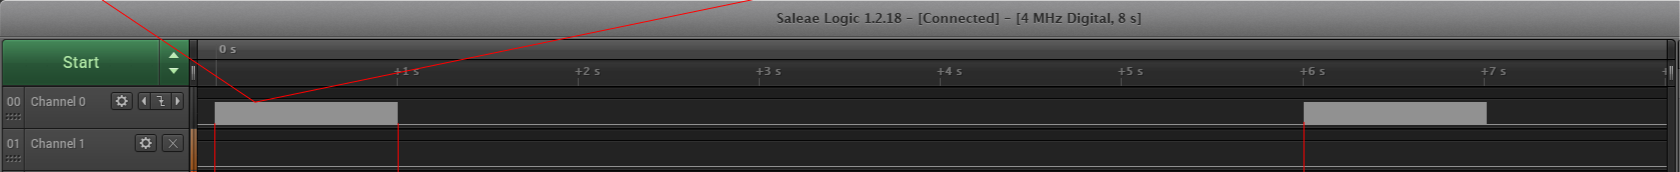
\includegraphics[width=\unitlength]{Bilder/Heating_PWM}}%
    \put(0.14,0.015){\color[rgb]{0,0,0}\makebox(0,0)[lt]{\begin{minipage}{0.00009384\unitlength}\centering Heizzeit\end{minipage}}}%
    \put(0.4,0.015){\color[rgb]{0,0,0}\makebox(0,0)[lt]{\begin{minipage}{0.15\unitlength}\centering inaktive Zeit\end{minipage}}}%
  \end{picture}%
\endgroup%
\caption{Logic Analyser Aufnahme vom Ausgang zur Heizungsansteuerung}
\end{figure}

 

